\documentclass[border=10pt]{standalone}

\usepackage{tikz}
\usepackage{tikzsymbols}
\usetikzlibrary{calc,patterns,shapes.geometric}

\def\centerarc[#1](#2)(#3:#4:#5){\draw[#1] ($(#2)+({#5*cos(#3)},{#5*sin(#3)})$) arc (#3:#4:#5);}

\begin{document}
	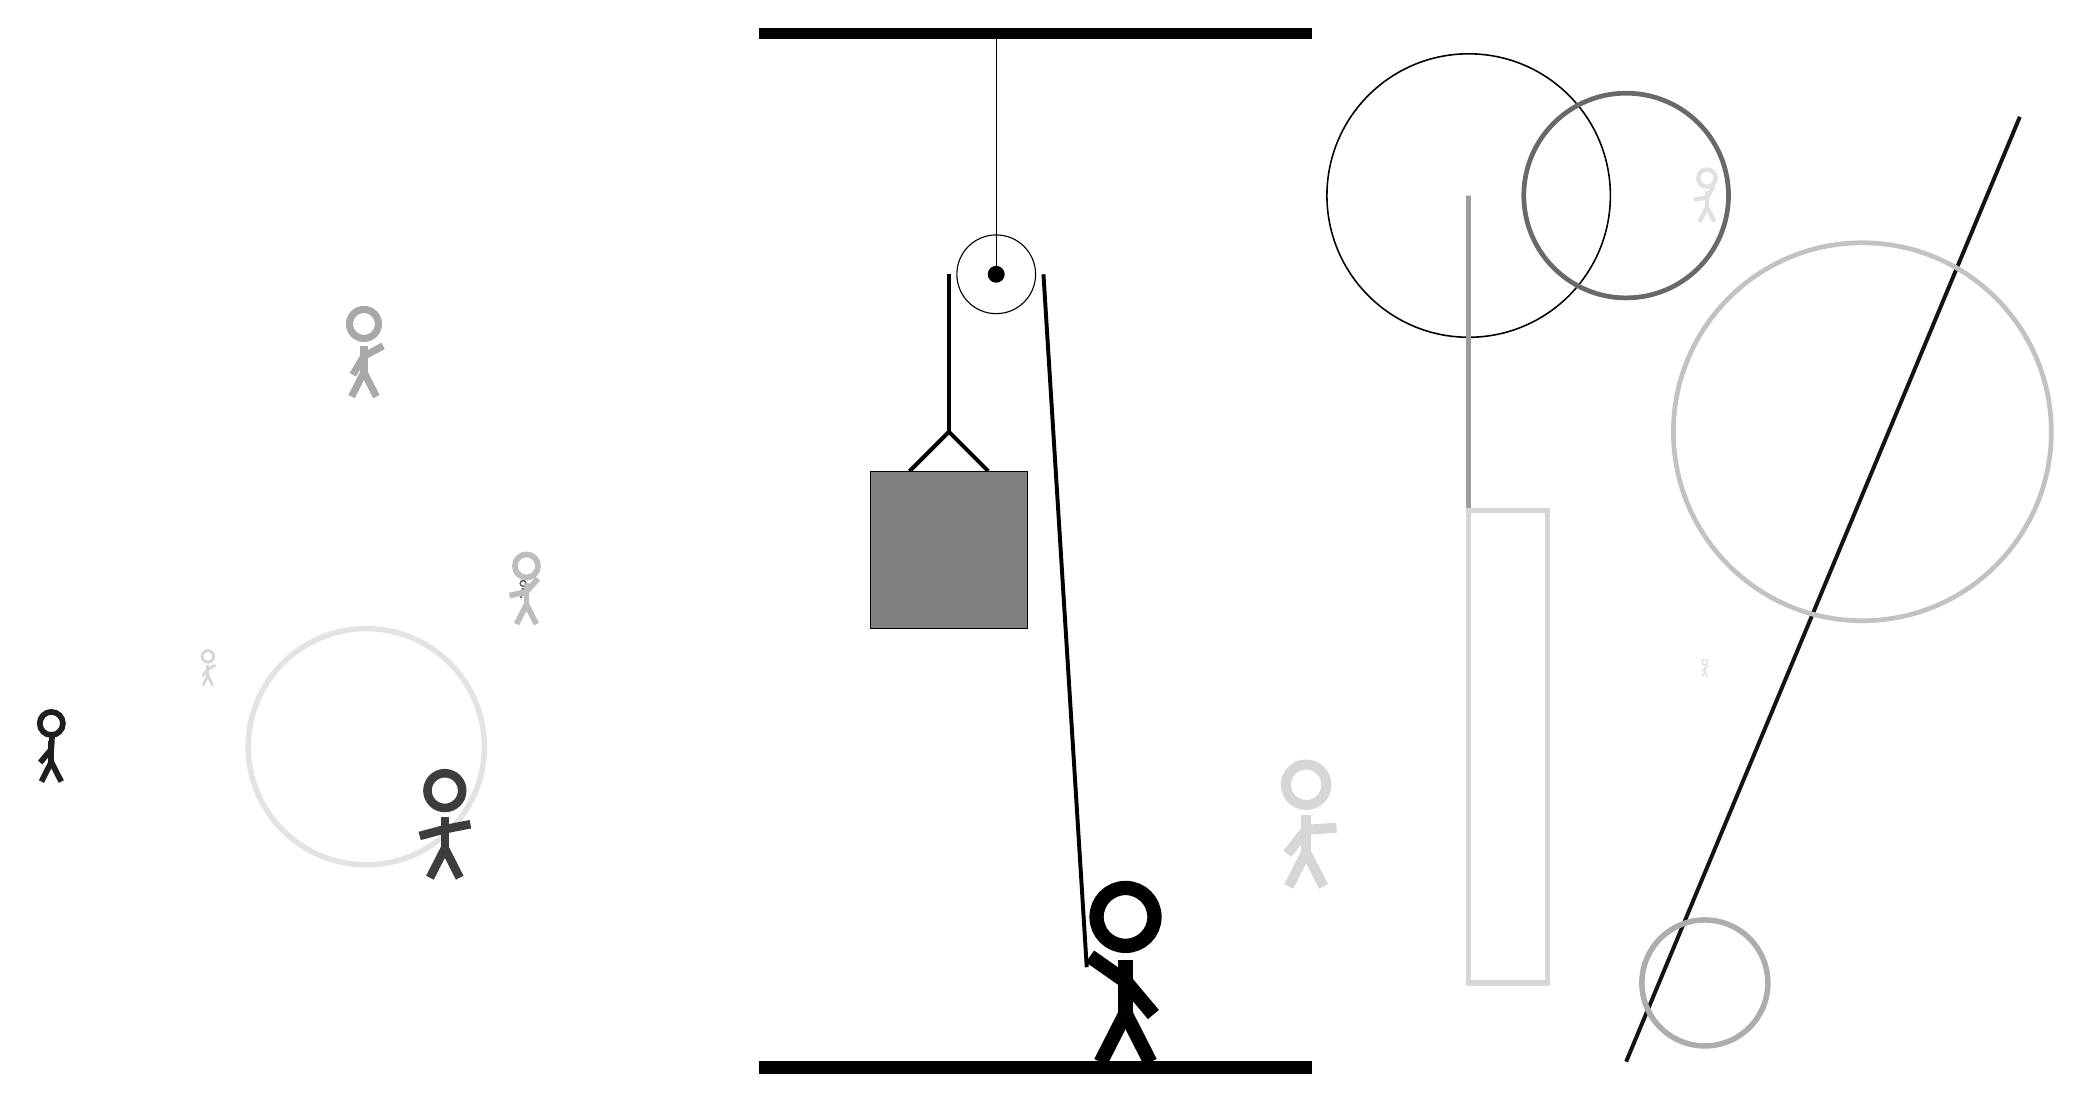
\begin{tikzpicture}
		%%%%% START %%%%%
		
		\draw[fill=black] (-2, 10) rectangle (5, 10.125);
		
		\draw (1, 7) circle (0.5);
		\draw[fill=black] (1, 7) circle (0.1);
		\draw (1, 10) -- (1, 7);
		
		\draw[line width=0.5mm] (-0.1, 4.5) -- (0.4, 5.0) -- (0.9, 4.5);
		\draw[fill=black!50] (-0.6, 4.5) rectangle (1.4, 2.5);
		
		\node[line width=0.2mm, color=black!63] at (-5, 3) {\Strichmaxerl[1][61][11]};
		
		\node[line width=0.3mm, color=black!88] at (-11, 1) {\Strichmaxerl[4][50][87]};
		\draw [line width=0.7mm, color=black!11](-7, 1) circle (1.5);
		\draw [line width=0.2mm, color=black!100](7, 8) circle (1.8);
		\node[line width=0.4mm, color=black!16] at (-9, 2) {\Strichmaxerl[2][52][28]};
		\node[line width=0.6mm, color=black!12] at (10, 2) {\Strichmaxerl[1][41][39]};
		\draw[line width=0.5mm, color=black!92](9, -3) -- (14, 9);
		\node[line width=0.6mm, color=black!16] at (5, 0) {\Strichmaxerl[7][52][4]};
		\node[line width=0.6mm, color=black!76] at (-6, 0) {\Strichmaxerl[6][15][11]};
		\draw[line width=0.6mm, color=black!39] (7, 3) rectangle (7, 8);
		\node[line width=0.4mm, color=black!34] at (-7, 6) {\Strichmaxerl[5][59][28]};
		\draw [line width=0.6mm, color=black!59](9, 8) circle (1.3);
		\node[line width=0.7mm, color=black!26] at (-5, 3) {\Strichmaxerl[4][13][49]};
		
		\node[line width=0.3mm, color=black!12] at (10, 8) {\Strichmaxerl[3][10][58]};
		\draw [line width=0.7mm, color=black!32](10, -2) circle (0.8);
		\draw [line width=0.6mm, color=black!24](12, 5) circle (2.4);
		
		\draw[line width=0.7mm, color=black!16] (7, 4) rectangle (8, -2);
		
		\draw[line width=0.5mm] (0.4, 7) -- (0.4, 5.0);
		\centerarc[line width=0.5mm](1, 7)(0:180:0.6);
		\draw[line width=0.5mm](1.6, 7) -- (2.15, -1.8);
		
		\node at (2.6, -1.9) {\Strichmaxerl[10][-35][-50]};
		
		\draw[fill=black] (-2, -3) rectangle (5, -3.15);
		
		%%%%% END %%%%%
	\end{tikzpicture}
\end{document}